\documentclass[11pt]{article}
\ifdefined\pdftrailerid\pdftrailerid{}\fi
\usepackage[T1]{fontenc}
\usepackage{lmodern}
\usepackage[letterpaper,margin=1in]{geometry}
\usepackage{amsmath,amssymb,amsthm,array,booktabs,microtype,tikz,xurl}
\definecolor{ink}{RGB}{23,76,87}
\definecolor{ochre}{RGB}{150,77,23}
\usepackage[colorlinks=true,allcolors=ink]{hyperref}
\hypersetup{pdftitle={Arithmetic certificates for normality and their limitations},pdfauthor={}}
\newtheorem{theorem}{Theorem}
\newtheorem{lemma}[theorem]{Lemma}
\newtheorem{proposition}[theorem]{Proposition}
\newtheorem{corollary}[theorem]{Corollary}
\newcommand{\R}{\mathbb R}
\newcommand{\Q}{\mathbb Q}
\newcommand{\Z}{\mathbb Z}
\newcommand{\T}{\mathbb T}
\newcommand{\circabs}[1]{\lVert #1\rVert_{\T}}
\DeclareMathOperator{\den}{den}
\newcommand{\baseurl}{https://github.com/eldernos/MathematicsResearch/blob/a09e011720bc74396a27f4cb3ce2d8a5b3ce5035}
\newcommand{\src}[3]{\href{\baseurl/NormalityChecker/#1.lean\#L#2}{#3}}
\setlength{\emergencystretch}{1.5em}
\raggedbottom

\begin{document}
\begin{center}
{\LARGE\bfseries Arithmetic certificates for normality\\and their limitations\par}
\vspace{0.6em}
{\small Technical report \enspace $\cdot$ \enspace 24 November 2026}
\end{center}
\begin{abstract}
We give a sufficient condition for normality in base \(b\) by approximating segments of the radix orbit in mean by rational orbits. The denominators grow on a proportion of segments tending to one, have prime factors in a fixed finite set coprime to \(b\), and are bounded by a fixed power of the segment length. The short exponential sum estimate used here is a qualitative consequence of Vandehey's theorem. If disjoint sets of positions have discrepancy at most \(\delta\) and cover a lower proportion \(g\), the limiting upper discrepancy is at most \(1-g(1-\delta)\). For a binary series supported on the primes \(2,5,13\), we enclose the upper density of simultaneous failures of two denominator tests within an interval of width \(10^{-10}\). We also prove that sufficiently accurate models on overlapping segments agree modulo one when their denominators satisfy the same support and size bounds on the overlap. On prescribed geometric schedules, the set of real numbers admitting arbitrarily accurate models has Lebesgue measure zero, even with unrestricted denominator primes.
\end{abstract}

\section{Rational approximations to digit shifts}
Let \(b\ge2\) be an integer. Write \(x_n=\{b^n x\}\in[0,1)\), \(e(t)=\exp(2\pi i t)\), and
\(\circabs{t}=\min_{m\in\Z}|t-m|\). For \(N\ge1\) set
\[
 D_N^{(b)}(x)=\sup_{0\le u<v\le1}
 \left|\frac1N\#\{0\le n<N:x_n\in[u,v)\}-(v-u)\right|,
 \qquad D_\infty^{(b)}(x)=\limsup_{N\to\infty}D_N^{(b)}(x).
\]
A real number is normal in base \(b\) if every word of length \(r\ge1\) has limiting frequency \(b^{-r}\), counting overlapping occurrences and using the terminating expansion at radix rationals. Each word corresponds to a half-open interval \([m/b^r,(m+1)/b^r)\), where \(0\le m<b^r\). Approximating both endpoints of any interval by points of this grid shows that normality is equivalent to \(D_N^{(b)}(x)\to0\). Write \(\den y\) for the positive denominator of \(y\in\Q\) in lowest terms. Call an integer \(Q\) supported on \(c\) if \(Q\mid c^j\) for some \(j\ge0\).

\begin{theorem}[Mean rational approximation]\label{thm:mean}
Fix \(b,c\ge2\) with \(\gcd(b,c)=1\), and integers \(L\ge2,\ B\ge1,\ d\ge0\). Let \(P_n\in\Q\) satisfy \(b^nx-P_n\to0\) in \(\R\). At scale \(k\ge0\) put
\[
 A=(LB)^k,\qquad T=B^k,\qquad m=L^k,\qquad A=mT.
\]
For each \(u=1,\ldots,LB-1\), integer \(M\ge1\) and \(\eta>0\), suppose that all sufficiently large \(k\) admit a set \(E\subseteq\{0,\ldots,m-1\}\) with \(|E|\le\eta m\) such that for every \(j\notin E\) in this range, writing \(n=uA+jT\), there exists a rational \(y\) with reduced denominator \(Q\) supported on \(c\) satisfying
\begin{equation}\label{eq:mean}
 M\le Q\le T^d,\qquad
 \frac1T\sum_{i=0}^{T-1}\circabs{P_{n+i}-b^i y}\le\eta .
\end{equation}
Then \(x\) is normal in base \(b\).
\end{theorem}

An \emph{arithmetic certificate} in this setting consists of the block models, the exceptional sets and the estimates in \eqref{eq:mean}, for fixed \(b,c,L,B,d\) and every \(M,\eta\). In the exact case \(y=P_n\) and \(P_{n+i}=b^iP_n\) throughout each retained block. If \(B=1\) or \(d=0\), then \(T^d=1\) precludes the hypotheses for \(M\ge2\) and \(\eta<1\). The real tail transfers character-sum bounds from \(P_n\) to the radix shifts.

Korobov studied digit frequencies on complete and incomplete periods of rational fractions \cite{korobov}. Bailey and Crandall relate radix recurrences with convergent perturbations to normality and use them in lacunary constructions \cite{bailey}. Vandehey obtains quantitative cancellation on a fixed finite prime support \cite[Cor.~1.2]{vandehey}. His Theorem~7.4 treats series \(\sum_j c_j^{-1}b^{-m_j}\) with \(c_j\) strictly increasing, \(c_j\mid c_{j+1}\), and a lower growth condition on \(m_j-m_{j-1}\). In Theorem~\ref{thm:mean} the denominator belongs to a model of a shifted prefix, where the sum of many coefficients may have undergone cancellation. The spacing condition is replaced by an estimate of the proportion of usable blocks.

For polynomial images of Stoneham numbers, the reduced denominator grows on the blocks between successive term insertions. In the localized logarithm with binary radix and support \(\{2,3\}\), rational phases with power-of-three denominators already yield a quantitative discrepancy estimate \cite[Thms.~1.1, 4.1]{localized}. Section~\ref{sec:joint} treats several independent denominator exponents by testing the same shifted prefix at different primes. The arithmetic of these two families is developed in the companion papers on \href{https://github.com/eldernos/MathematicsResearch/blob/3545d5f3072502e41d633d8900f20ad96c36be64/papers/01-stoneham-polynomials/paper.pdf}{Stoneham polynomial images} and \href{https://github.com/eldernos/MathematicsResearch/blob/3545d5f3072502e41d633d8900f20ad96c36be64/papers/02-localized-normality/paper.pdf}{localized polylogarithms}. For signed Stoneham expansions the uncovered positions can themselves be localized near zero on the circle. The discrepancy at cutoff \(N\) then differs from the fraction of positions in zero-phase shells by \(o(1)\), as proved in the \src{SignedShellDiscrepancy}{144}{signed-shell theorem} and developed in the \href{https://github.com/eldernos/MathematicsResearch/blob/3545d5f3072502e41d633d8900f20ad96c36be64/papers/03-signed-resonance/paper.pdf}{companion paper on signed expansions}.

\section{Short sums on a fixed prime support}
\begin{theorem}[Fixed-support estimate, after Vandehey]\label{thm:short}
For \(b,c\ge2\) coprime, each integer \(d\ge0\) and each \(\epsilon>0\), there is \(M=M(b,c,d,\epsilon)\) such that for every \(T\ge1\), \(y=a/Q\) in lowest terms with \(Q\) supported on \(c\) and \(M\le Q\le T^d\),
\[
 \left|\frac1T\sum_{i=0}^{T-1}e(b^iy)\right|\le\epsilon .
\]
\end{theorem}
For \(d>0\) the range is \(T\ge Q^{1/d}\). Vandehey's Corollary~1.2 gives \(O_{b,c,d}(Q^{-\sigma}(1+\log Q))\) for the displayed mean, for some \(\sigma>0\). His sum starts at exponent one, an equivalent convention since \(b\) permutes the reduced numerators. The following differencing argument proves this qualitative consequence directly.

\begin{proof}
Let \(r=\varphi(c^2)\) and \(C=b^r-1\). For each \(p\mid c\) and \(m\ge1\),
\[
 v_p(b^{rm}-1)=v_p(C)+v_p(m).
\]
Indeed \(p\mid C\) by Euler's theorem, and \(4\mid C\) if \(2\mid c\). For \(p\mid z\) (and \(4\mid z\) at \(2\)), the binomial expansion of \((1+z)^p-1\) gives valuation \(v_p(z)+1\). For \(p\nmid u\), the same expansion gives \(v_p((1+z)^u-1)=v_p(z)\). Iteration proves the formula. For \(Q>1\), let \(v_Q\) denote the order of \(b\) modulo \(Q\). Then \(Q\mid b^{rv_Q}-1\), hence \(Q\mid C v_Q\). In particular \(Q/C\le v_Q\le Q\).

Let \(G\) be the subgroup generated by \(b\) modulo \(Q\). Its Fourier sums satisfy
\[
 S(a)=\sum_{t\in G}e(at/Q),\qquad \sum_{a\bmod Q}|S(a)|^2=Qv_Q
\]
by character orthogonality. For a unit \(a\), \(S\) is constant on the \(v_Q\) points in \(aG\), so \(|S(a)|\le\sqrt Q\). Splitting into complete periods and a remainder yields
\begin{equation}\label{eq:period}
 \frac1T\left|\sum_{i<T}e(b^iy)\right|\le \frac{C}{\sqrt Q}+\frac{Q}{T}.
\end{equation}
Here and below \(i<T\) means \(0\le i<T\).

We prove uniform convergence to zero when \(K,Q\to\infty,\ T\ge K^3,\ Q\le K^s\), for each integer \(s\ge2\). Equation~\eqref{eq:period} proves the case \(s=2\). Suppose the assertion holds for \(s\) and consider \(K^s<Q\le K^{s+1}\). Multiply successive prime factors of \(Q\), with multiplicity, until their product \(D\) first reaches \(K\). Then \(D\mid Q\) and \(K\le D\le cK\). Write \(v=v_D\). For integers \(0\le j<l<H\) the difference of the translated phases \((b^{lv}-b^{jv})y\) has denominator \(Q/g\), where
\[
 g=\gcd(Q,b^{(l-j)v}-1),\qquad D\mid g,\qquad g\le C(l-j)v\le CHcK.
\]
The last bound follows since \(v_g\mid(l-j)v\) and \(g\le C v_g\). Consequently \(Q/g\le K^s\), while \(Q/g>K^{s-1}/(CHc)\) grows for fixed \(H\).

Set \(z_i=e(b^iy)\). The mean of \(z_{i+jv}\) over \(i<T\) differs from that of \(z_i\) by at most \(2Hv/T\). Average over \(0\le j<H\) and apply Cauchy--Schwarz in \(i\). The squared modulus of the translated mean is bounded by
\[
 \frac1H+\frac2{H^2}\sum_{0\le j<l<H}
       \left|\frac1T\sum_{i<T} z_{i+lv}\overline{z_{i+jv}}\right| .
\]
Each inner mean tends uniformly to zero by the induction hypothesis at denominator \(Q/g\). The translation error tends to zero since \(v\le cK\). Taking the upper limit first and then \(H\to\infty\) proves the induction step. Finally take \(K=\lfloor T^{1/3}\rfloor\). If \(d\ge1\) and \(Q\to\infty\), then \(K\to\infty\) and \(T^d\le K^{4d}\) for large \(K\). The case \(d=0\) is vacuous with \(M=2\).
\end{proof}

\begin{proof}[Proof of Theorem~\ref{thm:mean}]
Fix a nonzero integer \(h\). The denominator of \(hy\) is \(Q/\gcd(Q,|h|)\), between \(Q/|h|\) and \(Q\). Apply Theorem~\ref{thm:short} with tolerance \(\eta\) and choose the floor in \eqref{eq:mean} at least \(|h|\) times its threshold. For any \(s,t\in\R\),
\[
 |e(hs)-e(ht)|\le 2\pi |h|\,\circabs{s-t}.
\]
Thus a good full block contributes at most \((1+2\pi |h|)\eta T\) to the modulus of the \(h\)-sum for \(P\). More generally, if model sums are at most \(\epsilon T\), mean errors are at most \(\delta\), and \(E\) is the exceptional set of block indices, then at every cut \(0\le t\le mT\)
\begin{equation}\label{eq:prefix}
 \left|\sum_{i<t}e(h P_{uA+i})\right|
 \le(\epsilon+2\pi |h|\delta)mT+(|E|+1)T .
\end{equation}
In fact, each exceptional full block and the unfinished last block contributes at most \(T\) to the absolute sum.

Since \(T/A=L^{-k}\to0\), \eqref{eq:prefix} bounds every partial cell sum by \(o(A)\), uniformly in the finitely many \(u\), on letting \(\eta\downarrow0\). For a prefix ending in the shell \([A,(LB)A)\), sum over its earlier shells and its completed or partial cells. From any fixed large scale onward, an upper bound \(\rho (LB)^j\) per cell contributes at most \(\rho (LB-1)\sum_{j=0}^k (LB)^j\le \rho LB\,A\). Earlier positions contribute a bounded term. Divide by the prefix length, at least \(A\), and send \(\rho\) to zero. The character means for \(P_n\) therefore vanish. Those for \(b^nx\) have the same limit by the tail hypothesis and the Lipschitz bound. Weyl's criterion \cite{weyl} proves normality.
\end{proof}

\section{Coverage and overlapping intervals}\label{sec:cover}
For a nonempty finite set \(F\) of positions and a half-open test interval \(I\subset[0,1)\), write
\[
 C_I(F)=\sum_{i\in F}(\mathbf1_I(x_i)-|I|),\qquad
 D(F)=\frac{1}{|F|}\sup_I |C_I(F)|.
\]
The following estimates apply to any observations \(x_i\in[0,1)\). They need no arithmetic hypothesis on the pieces.

\begin{proposition}[Partial coverage]\label{prop:cover}
Suppose disjoint pieces in \([0,N)\) cover \(G\) positions altogether and each nonempty piece has discrepancy at most \(\delta\in[0,1]\). Then
\begin{equation}\label{eq:covered}
 D_N\le 1-(1-\delta)G/N .
\end{equation}
If, for every \(\epsilon>0\) and all sufficiently large \(N\), such pieces can be chosen with \(G/N\ge g-\epsilon\), then \(D_\infty\le1-g(1-\delta)\). More generally let \(F_N\subset[0,N)\) with \(\liminf |F_N|/N\ge g\). If \(\sup_I|C_I(F_N)|=o(N)\), then \(D_\infty\le1-g\).
\end{proposition}
\begin{proof}
On a piece \(F\), the centered sum has absolute value at most \(\delta |F|\). An uncovered position contributes at most one in absolute value since \(|\mathbf1_I-|I||\le1\). Add over the disjoint pieces and the remainder, then divide by \(N\) and take the supremum. The asymptotic inequality follows on letting \(\epsilon\downarrow0\). In the last assertion the two analogous costs are \(o(N)\) and \(N-|F_N|\).
\end{proof}
A fixed digit resolution has a different effect. If each of the \(q\ge1\) equal mesh intervals has limiting frequency \(1/q\), every union of consecutive mesh intervals has its correct limiting frequency, uniformly over this finite list. For each test interval, the circumscribed grid interval exceeds its length by at most \(2/q\), and the inscribed one falls short by at most \(2/q\). Hence \(D_\infty\le2/q\). In particular a test at one resolution gives a discrepancy bound even when finer resolutions have yet to be controlled.

\begin{proposition}[Endpoint paths]\label{prop:path}
Let \(f_i\) take values in a normed abelian group, with \(\|f_i\|\le1\), and let \(S(n)=\sum_{i<n}f_i\). Give an undirected edge between \(a\) and \(b'\) a cost \(w\) whenever \(\|S(b')-S(a)\|\le w\). Then
\[
 \|S(N)-S(0)\|\le\sum_{j=1}^m w_j
\]
on any path from \(0\) to \(N\) with successive edge costs \(w_j\). If an interval of length \(l+t+r\) has cost \(w\), its middle subinterval of length \(t\) has cost at most \(\min(t,w+l+r)\). For \(D_N\), it suffices that for each \(I\) there is a path of cost at most \(DN\) for \(f_i=\mathbf1_I(x_i)-|I|\). The path may depend on \(I\). The same bound on a complex sum applies to \(f_i=e(hx_i)\).
\end{proposition}
\begin{proof}
The telescoping sum for \(S(N)-S(0)\) uses a negative sign whenever an edge is traversed backwards. The triangle inequality gives the path cost. To restrict an edge, traverse the left discarded interval backwards, then the full edge, then the right discarded interval backwards. The discarded edges have costs at most \(l,r\), and directly summing over the middle gives \(t\). For centered counts divide by \(N\) and take the supremum over \(I\).
\end{proof}
For example, three consecutive runs \(+1,-1,+1\) of the same length \(T\) give zero sums on both overlapping intervals of length \(2T\). Their union has sum \(T\). In the opposite direction, zero sums on \([0,8),[2,8),[2,10)\) force the sum on \([0,10)\) to vanish by the path with vertices \(0,8,2,10\).

There is an exact interpretation of the shortest path when only scalar edge bounds are known. Include a unit-cost edge between every two consecutive indices in a finite range containing \(0,N\). If \(d(j)\) is the shortest path distance from \(0\), set \(f_i=d(i+1)-d(i)\). Then \(|f_i|\le1\) and \(|d(j)-d(k)|\le w\) on every given edge of cost \(w\). These data attain \(S(N)=d(N)\). Additional information about the particular characters or centered counts can give a smaller bound.

\section{Joint denominator tests at several primes}\label{sec:joint}
Let \(S\) be a finite set of primes. Write \(\mathcal M(S)\) for the positive integers supported on \(S\), including \(1\). For an integer \(s\ge1\) put
\[
 X=\sum_{m\in\mathcal M(S)}\frac{b^{-m}}{m^s},
 \qquad R_n=\sum_{\substack{m\in\mathcal M(S)\\m\le n}}\frac{b^{n-m}}{m^s}.
\]
For \(p\in S\) with \(p\nmid b\), choose a precision \(L_p\ge1\). Put \(w_p=(b^{-1})^{p^{L_p-1}}\bmod p^{L_p}\) and define on \(1\le t<p\)
\begin{equation}\label{eq:res}
 U_p(t)=\sum_{\substack{i\ge0\\is<L_p}} p^{is}
   \sum_{\substack{r\in\mathcal M(S\setminus\{p\})\\r\le p^i t}}
     r^{-s}w_p^r \pmod {p^{L_p}} .
\end{equation}
The inverses exist modulo \(p^{L_p}\). The failed region \(Z_p=\{t:U_p(t)=0\}\) is a finite union of half-open intervals. For \(n\ge1\) put \(k_p(n)=\lfloor\log_p n\rfloor\), \(t_p(n)=n/p^{k_p(n)}\) and \(B_p=\{n\ge1:t_p(n)\in Z_p\}\). For \(E\subseteq\Z_{\ge1}\), let \(\overline d(E)=\limsup_{N\to\infty}\#(E\cap[1,N))/N\).

\begin{theorem}[Joint failures at fixed precisions]\label{thm:joint}
For each nonempty \(J\subseteq\{p\in S:p\nmid b\}\) and any fixed choices of \(L_p\) for \(p\in J\),
\begin{equation}\label{eq:joint}
 D_\infty^{(b)}(X)\le \overline d\left(\bigcap_{p\in J}B_p\right).
\end{equation}
\end{theorem}
\begin{proof}
Fix \(p\in J\), let \(L=L_p\), and write \(k=k_p(n)\). Expand \(p^{ks}b^{-n}R_n\) by writing \(m=p^{k-i}r\), \(p\nmid r\). Row \(i\) carries the factor \(p^{is}\) and the cutoff \(r\le p^it_p(n)\). Euler's theorem gives \(w_p^p=w_p\bmod p^L\). If \(k\ge2(L-1)\), then \(k-i\ge L-1\) for all \(is<L\), so the factor \(b^{-p^{k-i}r}\) in those rows reduces to \(w_p^r\). All other rows vanish modulo \(p^L\). This proves \eqref{eq:res} is the residue of \(p^{ks}b^{-n}R_n\). At a passing position \(v_p(\den R_n)\ge ks-L+1\) for \(ks\ge L-1\). For any prescribed \(M\) the denominator is consequently at least \(M\) at all sufficiently late positions passing any test, since \(J\) is finite.

Following the block decomposition for the localized logarithm \cite[\S5]{localized}, take for each large \(N\) the length \(T=\lfloor\sqrt N\rfloor\). Partition its prefix into consecutive blocks of length \(T\), discarding the remainder, the initial block and each block \([a,a+T)\) for which \([a-T,a+T]\) contains an index from \(\mathcal M(S)\). Each index discards at most three full blocks. Up to \(N+T\) there are at most \((1+\log_2(N+T))^{|S|}\) such indices, by their exponent vectors. The discarded part contains \(o(N)\) positions. On a retained block,
\(R_{a+i}=b^iR_a\) for \(i<T\). Also \(0\le b^nX-R_n\le(n+1)^{-s}/(b-1)\), uniformly small for \(n\ge T\).

Let \(c=\prod_{p\in S,\,p\nmid b}p\) and \(H=\lceil\log_2(N+T)\rceil\). For \(m\le a\), \(m\in\mathcal M(S)\), one has \(m^s\mid b^{sH}c^{sH}\). The retained-block condition gives \(a-m\ge T\) for each such summand. Once \(T\ge sH\), its reduced denominator divides \(c^{sH}\), hence so does \(\den R_a\). Since \(c,s\) are fixed this common denominator is at most \(T^d\) for a fixed integer \(d\) and all large \(N\).

On a retained block containing a passing position, \(\den R_{a+i}\mid\den R_a\), so the starting denominators grow uniformly as \(N\to\infty\). Theorem~\ref{thm:short}, reduction after multiplication by each fixed \(h\ne0\), and the real tail bound give vanishing character means uniformly on these blocks. Their discrepancies tend uniformly to zero. Indeed, if uniform convergence failed, some sequence of these blocks would have discrepancy bounded below by a positive constant. Trigonometric polynomial approximation gives convergence of their empirical measures to Lebesgue measure on the circle, first on continuous functions and then on each interval of a fixed finite mesh by continuous upper and lower approximations. Inscription and circumscription on arbitrarily fine meshes give a contradiction. Each remaining full block consists entirely of joint failures. Proposition~\ref{prop:cover} now bounds \(N D_N^{(b)}(X)\) by the number of joint failures in the prefix plus \(o(N)\), proving \eqref{eq:joint}.
\end{proof}

The full unsigned classification in the \href{https://github.com/eldernos/MathematicsResearch/blob/3545d5f3072502e41d633d8900f20ad96c36be64/papers/02-localized-normality/paper.pdf}{companion paper on localized polylogarithms} already gives normality when \(J\) is nonempty. The fixed-precision bound above also quantifies how much of an orbit these particular tests certify before one passes to a limit in precision.

\subsection*{Two primes on logarithmic scales}
For a fixed pair \(p\ne q\) as above, define
\[
 a_p=\frac1{\log p}\int_{Z_p}\frac{dt}{t}.
\]
The logarithmic density of \(B_p\cap B_q\) is \(a_pa_q\). Indeed substitute \(y=e^z\) in the logarithmic integral through \(N\). The pair \((z/\log p,z/\log q)\bmod1\) is uniformly distributed in continuous time on the two-torus. Every nonconstant integer character has a nonzero frequency, since \(\log p/\log q\) is irrational. Integrating the character explicitly and approximating rectangles gives the product of their Haar measures. Replacing the integral by \(\sum_{n<N,\,n\in B_p\cap B_q}1/n\) incurs bounded error. Within each unit interval free of jumps the error is \(O(1/n^2)\). Near a jump it is \(O(1/n)\), summable along the finitely many geometric endpoint sequences.

Partial summation bounds this logarithmic density above by \(\overline d(B_p\cap B_q)\). Thus the product of logarithmic masses supplies a \emph{lower} bound on the cost on the right of \eqref{eq:joint}. Along nested refinements with positive limiting masses at both primes, that cost stays positive. Conversely, if \(a_p\to0\) then \(|Z_p|\le p(\log p)a_p\to0\). Summing the lengths of all completed and partial \(p\)-shells up to \(N\) gives \(\overline d(B_p)\le p|Z_p|/(p-1)\) at each fixed precision. In this case the single-prime test suffices in the limit. This two-prime calculation uses only the failure sets. It gives no lower bound on the discrepancy of \(X\).

\subsection*{A worked binary example}
Take \(b=2,\ S=\{2,5,13\},\ s=1\). At precision one only \(i=0\) contributes to \eqref{eq:res}. For \(p=5\), the cofactors below 5 are \(1,2,4\). The partial residues \(3,0,4\bmod5\) give \(Z_5=[2,4)\). For \(p=13\), the cofactors \(1,2,4,5,8,10\) give successive residues \(7,12,11,8,10,0\bmod13\), hence \(Z_{13}=[10,13)\). The individual upper densities are \(5/8\) and \(1/4\). At the end of a band \([ap^j,ep^j)\), the accumulated fraction tends to \(p(e-a)/(e(p-1))\), and between such endpoints the fraction first decreases and then increases.

To compute the upper density \(D_{\rm fail}\) of their intersection, extend both families of bands to all integer exponents on the positive real axis. This changes their mass below 1 by at most one. At integer cutoffs the counts above 1 equal lengths, since all the original endpoints are integers. On a component of the intersection the accumulated fraction is nondecreasing, and in the next gap it is nonincreasing. Its upper limit can therefore be computed at right endpoints of components, each a right endpoint of at least one family. Divide all coordinates by such an endpoint. If the fixed band is \([a,e)\) for the prime \(p\), its scaled copies are \(p^{-j}[a/e,1)\), \(j\ge0\). The other prime \(q\) contributes \(u q^{-j}[a',e')\), \(j\ge0\), with \(1/q\le u\le1\), clipped to \([0,1]\). The phases \(u\) approached at successive fixed endpoints are dense in this range by irrationality of \(\log p/\log q\).

Discard \([0,\tau)\), with \(0<\tau<1\). Only finitely many copies remain. Each intersection length is an affine function of \(u\) between crossings of moving endpoints with fixed endpoints (including the clipping boundaries). Its maximum therefore occurs at one of these finitely many ratios or at a phase endpoint. The sum is continuous there. If \(m_\tau\) is the larger of the two anchor maxima, density of the phases and a tail of length at most \(\tau\) give
\[
 m_\tau\le D_{\rm fail}\le m_\tau+\tau .
\]
For \(\tau=10^{-10}\), the two maxima, for anchors 5 and 13 respectively, are
\[
 \frac{147939288193417}{637289625781250},\qquad
 m_\tau=\frac{24154414499397933}{103559564189453125}.
\]
Thus \(D_{\rm fail}\) rounds to \(0.233241755\) at nine decimal places. This is a rational enclosure obtained by finite enumeration. A separate kernel proof bounds the number of joint failures in \([0,N)\) by \(0.234N+2197\) for every \(N\). The logarithmic density of the same failures is \((\log 2/\log 5)(\log(13/10)/\log13)\), about \(0.0441\). Ordinary density does not exist. The count stays constant from \(13^k\) to \(10\cdot13^k\), which rules out a positive density, while the positive logarithmic density rules out density zero.

\begin{figure}[htbp]
\centering
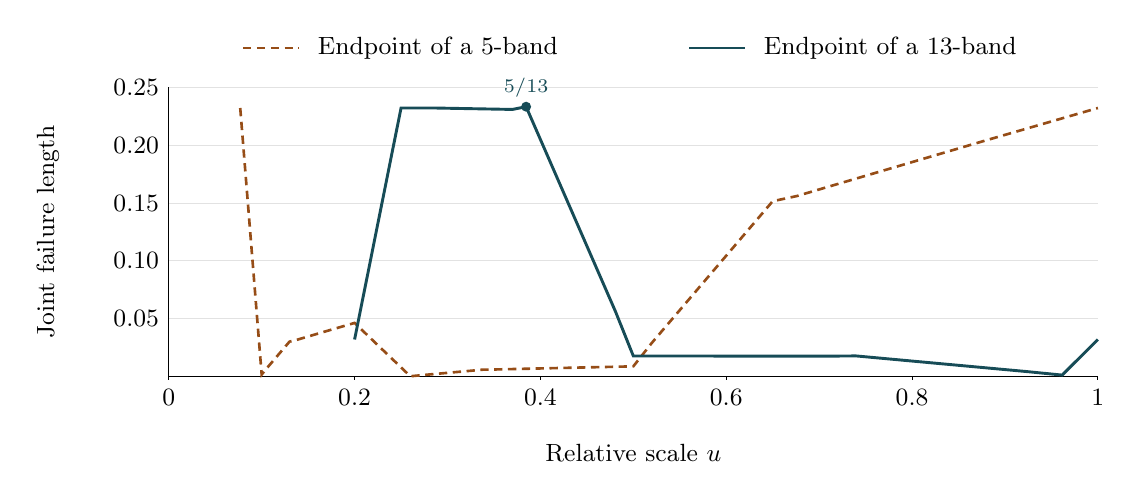
\begin{tikzpicture}[x=11.8cm,y=14.7cm,font=\small,
  anchorFive/.style={color=ochre,densely dashed,line width=0.95pt},
  anchorThirteen/.style={color=ink,line width=1.05pt}]
  \foreach \y in {0.05,0.10,0.15,0.20,0.25}{
    \draw[gray!23] (0,\y)--(1,\y);
    \node[left] at (0,\y) {\pgfmathprintnumber[fixed,precision=2,fixed zerofill]{\y}};}
  \draw (0,.25)--(0,0)--(1,0);
  \foreach \x in {0,0.2,0.4,0.6,0.8,1}{
    \draw (\x,0)--++(0,-.003);
    \node[below=1pt] at (\x,0){\pgfmathprintnumber{\x}};}
  \node[rotate=90] at (-.13,.125){Joint failure length};
  \node[anchor=north] at (.5,-.050){Relative scale \(u\)};
  \draw[anchorFive] plot coordinates {
(0.076923077,0.232137742)
(0.091395200,0.087680000)
(0.100000000,0.001785652)
(0.104000000,0.005857078)
(0.130000000,0.030321347)
(0.135200000,0.031214201)
(0.140608000,0.032494769)
(0.175760000,0.040802462)
(0.182790400,0.042432000)
(0.200000000,0.046426946)
(0.260000000,0.000355030)
(0.270400000,0.001169231)
(0.285610000,0.002270000)
(0.338000000,0.006063373)
(0.351520000,0.006242308)
(0.365580800,0.006498800)
(0.371293000,0.006602800)
(0.456976000,0.008160492)
(0.475255040,0.008486400)
(0.500000000,0.008928259)
(0.520000000,0.029285389)
(0.650000000,0.151606736)
(0.676000000,0.156071006)
(0.703040000,0.162473846)
(0.878800000,0.204012308)
(0.913952000,0.212160000)
(1.000000000,0.232137742)
};
\draw[anchorThirteen] plot coordinates {
(0.200000000,0.032142809)
(0.210413339,0.073796166)
(0.250000000,0.232137742)
(0.273537341,0.232134729)
(0.284478835,0.232148734)
(0.355598543,0.231101852)
(0.369822485,0.230874269)
(0.384615385,0.233241133)
(0.480769231,0.056318056)
(0.500000000,0.017856518)
(0.526033348,0.017856518)
(0.547074682,0.017857595)
(0.683843353,0.017777066)
(0.711197087,0.017759559)
(0.739644970,0.017941626)
(0.924556213,0.004332158)
(0.961538462,0.001373578)
(1.000000000,0.032142809)
};
\coordinate (jointPeak) at (0.384615385,0.233241133);

  \fill[ink] (jointPeak) circle[radius=1.8pt];
  \node[above,font=\scriptsize,ink] at (jointPeak) {\(5/13\)};
  \draw[anchorFive] (.08,.284)--(.14,.284);
  \node[right] at (.15,.284){Endpoint of a 5-band};
  \draw[anchorThirteen] (.56,.284)--(.62,.284);
  \node[right] at (.63,.284){Endpoint of a 13-band};
\end{tikzpicture}
\caption{Exact finite computation for the binary support \(\{2,5,13\}\) at precision one. The curves give the joint failed length in \([10^{-5},1]\) after rescaling a right endpoint to 1. The parameter \(u\) sets the relative scale of the other prime\textquoteright s bands. The dashed curve starts at \(1/13\), the solid curve at \(1/5\). The solid peak occurs at \(u=5/13\), where the newest left endpoints coincide at \(10/13\).}\label{fig:curves}
\end{figure}

At precision two both primes have empty failed regions. For example, the \(i=0,1\) rows modulo 25 change only at \(t=1,8/5,2,13/5,16/5,4\), where their combined residues are respectively \(13,23,10,15,20,14\). For \(p=13\) checking the grid \(t=j/13\), \(13\le j<169\), includes all cell boundaries. The smallest and largest residues are 7 and 167. Theorem~\ref{thm:joint} now gives \(D_\infty^{(2)}(X)=0\). Thus a positive upper density of failures at the first precision is compatible with zero limiting discrepancy.

\section{Separation on a shared segment}\label{sec:rigidity}
\begin{theorem}[Uniform separation]\label{thm:rigidity}
Fix coprime integers \(b,c\ge2\) and an integer \(d\ge0\). There exists \(\gamma=\gamma(b,c,d)>0\) with the following property. Suppose \(T\ge1\), \(y,z\in\Q\) have reduced denominators supported on \(c\) and at most \(T^d\), and \(y-z\notin\Z\). For any real observations \(f_0,\ldots,f_{T-1}\),
\begin{equation}\label{eq:rigid}
 \frac1T\sum_{i<T}\big(\circabs{f_i-b^iy}+\circabs{f_i-b^iz}\big)\ge\gamma .
\end{equation}
\end{theorem}
\begin{proof}
Put \(w=y-z\) and \(Q=\den w>1\). Then \(Q\) divides \(\den(y)\den(z)\), so its support is fixed and \(Q\le T^{2d}\). Let \(M\ge2\) be the threshold of Theorem~\ref{thm:short} for \(2d\) and tolerance \(1/2\). If \(Q\ge M\), then
\[
 \frac T2\le \left|T-\sum_{i<T}e(b^iw)\right|
      \le 2\pi\sum_{i<T}\circabs{b^iw}.
\]
For \(1<Q<M\), every \(b^iw\) still has reduced denominator \(Q\), hence distance at least \(1/Q\) to the nearest integer. In either case the mean distance is at least \(\gamma=\min(1/M,1/(4\pi))\). Apply the circle triangle inequality through \(f_i\) at each position.
\end{proof}

\begin{corollary}[Overlapping models]\label{cor:chain}
Fix \(b,c,d\) as in Theorem~\ref{thm:rigidity}. For each \(j\) let \(T_j\ge1\), and let \(y_j,z_j\) have reduced denominators supported on \(c\) and at most \(T_j^d\). If for observations \(f^{(j)}_i\), \(0\le i<T_j\), the left side of \eqref{eq:rigid} for this pair tends to zero as \(j\to\infty\), then \(y_j-z_j\in\Z\) for all sufficiently large \(j\).

In particular, consider consecutive blocks with rational models \(y_j,y_{j+1}\), whose start indices differ by \(r_j\ge0\) and whose overlap has length \(T_j\ge1\). Suppose both denominators are supported on \(c\) and at most \(T_j^d\). If the combined mean error of the aligned models \(b^{r_j}y_j,y_{j+1}\) on their common observations tends to zero, then \(\den y_j\) is eventually constant.
\end{corollary}
\begin{proof}
Once the error is below \(\gamma\), \eqref{eq:rigid} forces integral difference. Multiplication by \(b^{r_j}\) preserves any denominator supported on \(c\), and an integer translation preserves it as well. Therefore \(\den y_{j+1}=\den y_j\) for all sufficiently large \(j\).
\end{proof}

Both the error and the size bound in this argument refer to the \emph{overlap}. Small mean error on a longer block can concentrate on its short shared part. A size bound polynomial in the original length suffices if that length is bounded by a fixed power of \(T\). Three examples distinguish the restrictions.

If a denominator shares a radix factor, the models \(0,1/b\) coincide after one shift. Their mean distance is \(1/(bT)\). Without the size bound, the fixed-support models \(0,c^{-T^2}\) have mean distance at most \(b^Tc^{-T^2}\to0\). Finally, for \(m\ge2\) put \(Q_m=b^m-1\) and take \(0,1/Q_m\) with \(T=mQ_m\). These denominators are prime to \(b\) and at most \(T\). Each length-\(m\) period has sum of the distances to zero at most \(\sum_{j<m} b^j/Q_m=1/(b-1)\). Their mean distance tends to zero, so arbitrary changes of prime support defeat uniform separation even with \(d=1\). The same example has first character mean tending to one. No fixed finite set of primes supports all these denominators since \(v_{Q_m}\le m\) and any fixed support would give \(Q_m\le C m\) in the proof of Theorem~\ref{thm:short}.

\section{A counting obstruction}\label{sec:count}
We bound the measure of points approximated on a prescribed block by any rational orbit whose denominator is bounded by a power of the block length. Let \(\lambda\) be Lebesgue probability measure on \([0,1)\).

\begin{theorem}[Polynomially many rational models]\label{thm:count}
Fix \(b\ge2,\ d\in\Z_{\ge0}\), put \(a=b^2\), and set \(\eta_b=1/(16a^2)\). For a prescribed start \(n\ge0\) and length \(T\ge2\), let \(E_{n,T}\) consist of all \(x\in[0,1)\) for which a rational \(y\) with \(\den y\le T^d\) satisfies \(T^{-1}\sum_{i<T}\circabs{b^{n+i}x-b^iy}\le\eta_b\). Then
\begin{equation}\label{eq:prob}
 \lambda(E_{n,T})\le T^{2d}\exp\!\left(-\frac{\lfloor T/2\rfloor}{4a}\right).
\end{equation}
Let \(T_k=B^k\) for an integer \(B\ge2\), with at most \(O(T_k^A)\) prescribed starts at each scale, for a fixed \(A\ge0\). For almost every \(x\) there is \(k_0(x)\) such that none of the prescribed starts admits such a model at any scale \(k\ge k_0(x)\).
\end{theorem}
\begin{proof}
Fix \(y\). Under \(\lambda\), \(z=\{b^n x-y\}\) is uniform. Its first \(J=\lfloor T/2\rfloor\) base-\(a\) digits form an equiprobable word, since each cylinder has length \(a^{-J}\). An occurrence of digit \(1\) in position \(j+1\), \(0\le j<J\), puts \(\{b^{2j}z\}\) in \([1/a,2/a)\), at distance at least \(1/a\) from an integer since \(a\ge4\). The mean error condition allows at most \(K=\lfloor a\eta_b T\rfloor\) such occurrences.

Give digit \(1\) weight one and every other digit weight two. The total product weight of all words is \((2a-1)^J\), while each word with at most \(K\) occurrences has weight at least \(2^{J-K}\). Its class has probability at most
\[
 2^K(1-1/(2a))^J \le \exp(-J/(4a)).
\]
Indeed \(T\le3J\) for \(T\ge2\), hence \(K\log2\le 3J\log2/(16a)\le J/(4a)\). There are at most \(\sum_{q\le T^d}q\le T^{2d}\) rational models modulo one. A union bound gives \eqref{eq:prob}. Multiplying by the number of starts leaves a summable sequence in \(k\). The first Borel--Cantelli lemma gives the assertion without independence between starts.
\end{proof}
The exponential estimate is a finite-word instance of the standard lower-tail estimate for independent digits (compare Hoeffding \cite{hoeffding}). Borel--Cantelli also applies simultaneously to a countable family of prescribed schedules. In particular the integer parameters \(b,B,L,d\) of Theorem~\ref{thm:mean} give only countably many schedules, with \((LB-1)L^k\) starts per scale. On a late block the real tail \(b^jx-P_j=o(1)\) changes its mean error by \(o(1)\) uniformly for \(j\) beyond the block start. An arbitrarily accurate certificate for \(P\) would therefore give an approximation in \eqref{eq:prob}. Borel's theorem gives normality for almost every \(x\) \cite{borel}. The numbers admitting these certificates form a null set. This measure estimate applies to prescribed schedules.

\section{Formal correspondence and sources}
The formal statements use the \src{Basic}{23}{digit-cylinder definition of normality} and the \src{BinaryDiscrepancy}{11}{supremum over half-open intervals}. In Theorem~\ref{thm:mean} the Lean statement takes the short-orbit estimate as an argument. Theorem~\ref{thm:short} supplies it for the \(b,c\) in the printed statement. For Proposition~\ref{prop:cover} the formal statement specializes the observations to radix orbits. For Theorem~\ref{thm:joint}, Lean indexes precision \(L_p\) by \(L_p-1\) and expresses the upper density hypothesis as a bound with arbitrarily small slack for every late prefix. Theorem~\ref{thm:count} uses a formal finite word count. The measure estimate, the two-prime logarithmic density, the sharpness statement for scalar edge data, and the rational enclosure in the worked example are proved or computed here on paper.

\begin{center}
\small
\begin{tabular}{@{}p{.32\linewidth}p{.63\linewidth}@{}}
\toprule
Printed result & Lean declaration at the proof revision\\ \midrule
Theorem~\ref{thm:mean} (AC-01) &
 \src{ArithmeticCertificate}{62}{\nolinkurl{normal_of_approximate_arithmetic_certificate}}\\
Theorem~\ref{thm:short} (AC-04), \eqref{eq:prefix} &
 \src{SmoothOrbit}{207}{\nolinkurl{fixed_support_orbit_estimate}}\newline
 \src{ArithmeticCertificate}{34}{\nolinkurl{approximate_prefix_bound}}\\
Proposition~\ref{prop:cover} (AC-02) &
 \src{QualityCoverage}{13}{\nolinkurl{Coverage.fixed_quality_cover}}\newline
 \src{QualityCoverage}{38}{\nolinkurl{Coverage.asymptotic_fixed_quality}}\newline
 \src{PartialUniformity}{75}{\nolinkurl{discrepancy_of_uniform_share}}\\
Proposition~\ref{prop:path} (AC-07) &
 \src{IntervalCoverage}{15}{\nolinkurl{Coverage.endpoint_path}}\newline
 \src{IntervalCoverage}{39}{\nolinkurl{Coverage.restrict_edge}}\newline
 \src{IntervalCoverage}{67}{\nolinkurl{Coverage.discrepancy_of_paths}}\\
Theorem~\ref{thm:joint} (AC-06) &
 \src{DiscrepancyChecker}{113}{\nolinkurl{LocalizedSupport.discrepancy_of_joint_failures}}\\
First-precision example &
 \src{DiscrepancyChecker}{141}{\nolinkurl{LocalizedSupport.five_thirteen_first_failures}}\newline
 \src{JointFiveThirteen}{114}{\nolinkurl{LocalizedSupport.joint_five_thirteen_count}}\\
Second-precision example &
 \src{DiscrepancyChecker}{153}{\nolinkurl{LocalizedSupport.five_thirteen_precision_two}}\newline
 \src{DiscrepancyChecker}{156}{\nolinkurl{LocalizedSupport.five_thirteen_binary_normal}}\\
Theorem~\ref{thm:rigidity}, Corollary~\ref{cor:chain} (AC-03) &
 \src{OrbitRigidity}{32}{\nolinkurl{smooth_overlap_separation}}\newline
 \src{OrbitRigidity}{83}{\nolinkurl{smooth_overlap_rigidity}}\newline
 \src{OrbitRigidity}{101}{\nolinkurl{overlap_chain_denominator}}\\
Theorem~\ref{thm:count} (AC-10), word inequality &
 \src{ModelCounting}{14}{\nolinkurl{few_symbol_words}}\\ \bottomrule
\end{tabular}
\end{center}
\noindent\begin{minipage}{\linewidth}
\subsection*{Source code and reproduction}
All displayed declaration names have the prefix \texttt{NormalityChecker.}
The links point to the immutable \href{https://github.com/eldernos/MathematicsResearch/tree/a09e011720bc74396a27f4cb3ce2d8a5b3ce5035}{formal source revision \texttt{a09e0117}}. The accompanying \nolinkurl{CORRESPONDENCE.md} includes the fully qualified names and supporting lemmas. From a built checkout, these commands check the statements and their allowed axioms, regenerate the rational data for Figure~\ref{fig:curves}, and compile this report.
\begin{small}
\begin{verbatim}
lake env lean papers/04-arithmetic-certificates/Check.lean
python3 -B papers/04-arithmetic-certificates/figures/joint_density.py
papers/build.sh 04-arithmetic-certificates
\end{verbatim}
\end{small}
\end{minipage}

\smallskip
\noindent\emph{AI assistance.} AI systems assisted the project owner with the exploration of rational orbit models, the development of the certificate and rigidity arguments, and their formalization in Lean. OpenAI Codex drafted the exposition, checked statement correspondence and prepared the figure and its data. Authorship and submission decisions remain with the project owner.

\begingroup\small
\bibliographystyle{plain}
\bibliography{references}
\endgroup
\end{document}
